\documentclass[a5paper, 11pt]{extarticle}
\usepackage[utf8]{inputenc}
\usepackage[T1]{fontenc}
\usepackage{graphicx}
\usepackage{longtable}
\usepackage{tabularray}
\usepackage{wrapfig}
\usepackage{rotating}
\usepackage{float}
\usepackage[normalem]{ulem}
\usepackage{amsmath}
\usepackage{amssymb}
\usepackage{capt-of}
\usepackage{hyperref}
\usepackage{fontspec}
\usepackage[russian]{babel}
\usepackage{indentfirst}
\setmainfont{PT Astra Serif}
\usepackage[
    left=10mm,
    right=10mm,
    top=15mm,
    bottom=15mm
]{geometry}
\usepackage{amsthm}
\usepackage{enumitem}
\usepackage{unicode-math}
\usepackage[math]{cellspace}
\usepackage{mathtools}

\pagestyle{plain}

\theoremstyle{definition}
\newtheorem{theorem}{Теорема}[section]
\renewcommand{\thetheorem}{\arabic{theorem}}

\newtheorem*{theorem*}{Теорема}

\newtheorem{lemma}{Лемма}[section]
\renewcommand{\thelemma}{\arabic{lemma}}

\newtheorem{property}{Свойство}[section]
\renewcommand{\theproperty}{\arabic{property}}

\theoremstyle{definition}
\newtheorem{definition}{Определение}[section]
\renewcommand{\thedefinition}{\arabic{definition}}

\theoremstyle{definition}
\newtheorem*{definition*}{Определение}

\newtheorem{consequence}{Следствие}[section]
\makeatletter
\counterwithin{consequence}{property}
\counterwithin{consequence}{theorem}
\makeatother
\renewcommand{\theconsequence}{\arabic{consequence}}

\newtheorem*{consequence*}{Следствие}

\newtheorem{note}{Замечание}[section]
\makeatletter
\counterwithin{note}{property}
\counterwithin{note}{theorem}
\makeatother
\renewcommand{\thenote}{\arabic{note}}

\newtheorem*{note*}{Замечание}

\numberwithin{figure}{section}


\newcommand{\newpar}{$ $\par\nobreak\ignorespaces}
\renewenvironment{proof}{{\noindent\bfseries Доказательство.}}{\smallskip\newpar \hfill\textit{Что и требовалось доказать.}}
\usepackage[x11names]{xcolor}
\hypersetup{linktoc = all, colorlinks = true, urlcolor = DodgerBlue4, citecolor = PaleGreen1, linkcolor = black}
\author{Daniil Shvalov}
\date{\today}
\title{}
\hypersetup{
    pdfauthor={Daniil Shvalov},
    pdftitle={},
    pdfkeywords={},
    pdfsubject={},
    pdflang={Russian}}


% Define math operators
\DeclareMathOperator{\rang}{rang}
\DeclareMathOperator{\Ima}{Im}
\DeclareMathOperator{\defect}{def}


% Draw line in matrix
\makeatletter
\renewcommand*\env@matrix[1][*\c@MaxMatrixCols c]{%
    \hskip -\arraycolsep
    \let\@ifnextchar\new@ifnextchar
    \array{#1}}
\makeatother

% Add new table align types
\newcommand{\PreserveBackslash}[1]{\let\temp=\\#1\let\\=\temp}
\newcolumntype{C}[1]{>{\PreserveBackslash\centering}p{#1}}

\setlist[itemize]{itemsep=0.5em,topsep=0em,parsep=0em}
\setlist[enumerate]{itemsep=0.5em,topsep=0em,parsep=0em}

\hypersetup{linktoc = all, colorlinks = true, urlcolor = DodgerBlue4, citecolor = PaleGreen1, linkcolor = blue}

\makeatletter
\def\thm@space@setup{\thm@preskip=1pt
    \thm@postskip=1pt}
\makeatother

\def\lets{%
    \mathord{\setbox0=\hbox{$\exists$}%
        \hbox{\kern 0.125\wd0%
            \vbox to \ht0{%
                \hrule width 0.75\wd0%
                \vfill%
                \hrule width 0.75\wd0}%
            \vrule height \ht0%
            \kern 0.125\wd0}%
    }%
}

\begin{document}

\hypersetup{linktoc = all, colorlinks = true, urlcolor = DodgerBlue4, citecolor = PaleGreen1, linkcolor = black}
\tableofcontents
\hypersetup{linktoc = all, colorlinks = true, urlcolor = DodgerBlue4, citecolor = PaleGreen1, linkcolor = blue}
\newpage

% Проблемы, связанные с экологией.

% Эпоха глобального экологического кризиса.

\section{Введение в экологию}

\subsection{Глобальный экологический кризис}

В связи с экспоненциальным ростом численности человечества, развитием техники и все большим стремлением к повышению уровня потребления у среднего жителя Земли к концу XX века возникли предпосылки экологического кризиса, то есть перехода биосферы к неустойчивому состоянию.

Кризисная ситуация усугубляется быстрым вымиранием видов живых организмов. В норме нормальные изменения условий в природе сопровождаются вымиранием одного вида за 100 лет, то в настоящее время всего за 1 час на Земле исчезает 50 видов. К концу XX века 63\% естественных экосистем суши разрушены, гибнут многие водные экосистемы.

Причины:
\begin{itemize}
    \item техногенное загрязнение окружающей среды (добыча полезных ископаемых, производство, ресурсный цикл);
    \item нерациональное использование природных ресурсов, распахивание земель;
    \item рост народонаселения (особенно в развивающихся странах);
    \item рост уровня потребления в развитых странах.
\end{itemize}

Разнокачественность системы -- это один из элементов ее устойчивости. Хуже всего адаптируются и перестраиваются простые системы, основанные на простых взаимодействиях. Выпадение элемента или нарушение какой-либо связи может привести к краху такой системы.

Примером системы может выступать агросистема. Один паразит может нарушить работу всей системы.

Большую часть времени человечество развивалось под эгидой антропоцентризма. Это привело к проблемам, с которыми приходится иметь дело в наши дни. Чтобы исправить положение, человечество должно придерживаться биоцентризма.

Качеством природной среды <<автоматически>> может управлять только биота, то есть совокупность всех живых организмов Земли. Биологическое разнообразие (разнообразие и количество видов, составляющих экосистему) является главным критерием и признаком устойчивости экосистемы.

Биота способна восстановить нормальную природную среду обитания, качество воды, воздуха, почвы, пищи, утерянные в результате экологического кризиса, но только в случае, если для восстановления самой биоты будут представлены время и место.

Сохранение биологического разнообразия возможно только в сообществах и в определенных условиях, поэтому для их сохранения необходимо выделение специально охраняемых территорий (заповедники), площадь которых на суше должна составлять не менее 1/6 ее части.

Искусственно создать среду обитания для человека не удается, что подтверждено многочисленными экспериментами в разных странах мира.

Экология -- это наука, изучающая взаимоотношения организмов между собой и с окружающей средой.

Экология -- это наука, изучающая взаимоотношения биологических систем разного ранга с окружающей средой (организм, популяция, сообщество или биоценоз).

Экосом греки называли любое место пребывания человека: пляж, где люди собирались для купания, горное пастбище, где пастухи пасли овец и др.

В середине XX века экологию стали понимать как науку об экосистемах и биосфере.

Начало такому понимаю положили работы В. И. Вернадского, В. В. Докучаева, Ю. П. Одума, А. Дж. Тенсли, Н. В. Тимофеева-Ресовского и других известных ученых.

Уровни организации живой материи:
\begin{enumerate}
    \item молекулы;
    \item протоплазма;
    \item клетки;
    \item ткани;
    \item органы;
    \item системы органов;
    \item организмы (тут начинается экология);
    \item популяции;
    \item сообщества;
    \item экосистемы;
    \item биосфера;
\end{enumerate}

\subsection{История становления экологии}

Экология как наука начала формироваться в конце XVIII века, сначала как один из разделов зоологии. Первые представления о биосфере как области жизни и оболочке Земли даны Ж. Б. Ламарком (1744 -- 1829).

Термин <<биосфера>> впервые ввел в научных обиход в 1875 году австрийский геолог Э. Зюсс (1831 -- 1914).

В работе Т. Мальтуса (1798) приведены уравнения экспоненциального роста популяции. П. Ф. Ферхюльст предложил уравнение <<логистического>> роста. Эти работы обосновали представления о динамике численности популяций.

Ю. Либих сформулировал правило <<лимитирующего фактора>>.

Термин <<экология>> впервые введен в 1866 году немецким биологом Э. Геккелем (1834 -- 1919).

\subsection{Системная парадигма в экологии}

Система -- это саморазвивающаяся и саморегулирующаяся, определенным образом упорядоченная материально-энергетическая совокупность, существующая и управляемая как относительно устойчивое единое целое за счет взаимодействия, распределения и перераспределения имеющихся, поступающих извне и продуцируемых совокупностью веществ, энергии и информации, и обеспечивающая преобладание внутренних связей (в т. ч. перемещений веществ, энергии и информации) над внешними.

Система -- это множество элементов, образующих определенную целостность, единство.

Элемент в рамках системы -- это неделимая ее часть. Для молекулы -- атом, для атома -- элементарная частица, для организма -- клетка, для клетки -- ядро, митохондрии и другие органеллы, для макромолекулы -- атом, для атома -- элементарная частица. Для экосистемы элементом является организм.

Движущей силой в любой материальной системе служит энергия. Ее основным источником на Земле является Солнце.

\subsection{Экология в системе естественных наук}

Современная экология -- это фундаментальная наука о природе, являющаяся комплексной и объединяющая знание основ естественных наук: биологии, геологии, географии, климатологии, ландшафтоведения и др.

Экологические системы, как и живые системы других уровней организации, являются сложными, характеризующимися нелинейной динамикой.

Согласно основным положениям экологии, человек как один из биологических видов, является частью биосферы и также, как и другие организмы, не может существовать без биоты, т. е. без совокупности живущих ныне на Земле биологических видов.

Основные методы экологических исследований: полевые (метод наблюдения), экспериментальные, лабораторные исследования, сравнительный метод, моделирование.

Прикладная цель экологии -- оптимизация взаимодействия челочка с природной на основе знания экологических законов.

\subsection{Экология как мировоззрение}

К концу XX века научный термин <<экология>> стал использоваться также для обозначения определенного типа мировоззрения, предполагающего бережное отношение к природе. Формируется биоцентрическое мировоззрение, сменяющее антропоцентрическое, в котором в центре природы и мироздания стоит человек, и от социоцентрического, в котором центром и целью жизни самого человека является тоталитарная социальная или производственная система.

Развитие концепции русской классической школы биологов и экологов, направленной на изучение явлений коэволюции к природе, и в том числе возможности сопряженной эволюции человека и биосферы. Это концепция разработана в трудах В. И. Вернадского (теория ноосферы), Н. В. Тиомфеева-Ресовского.

% oaliashenko@itmo.ru
% презентация не менее 10 слайдов
% текст можно помещать на слайды (желательно в сокращенном виде)
% первый слайд титульный
% оформление свободное
% преамбула -- формулировка проблемы, которую собираетесь освещать
% заключительная часть, выводы (собственное мнение приветствуется)
% последний слайд -- список использованных источников

% \section{Гидроэлектростанции и связанные с ними экологические проблемы}

% ГЭС, в которых необходимый напор воды обеспечивается посредством сооружения плотины и водохранилища и, как следствие, концентрации воды реки в определенном месте.

% \subsection{Этап строительства}

% Гидротехнические работы, как и любое строительство, негативно влияет на окружающую среду:
% \begin{itemize}
%     \item Интенсивное потребление воды (приготовление композиционных материалов, водоснабжение двигателей различных технологических установок, намыв грунта и т. д.).
%     \item Загрязнение водных объектов стоками со строительных площадок, веществами, выщелачиваемыми из бетона.
%     \item загрязнение вследствие использования инъекционных растворов для противофильтрационных и укрепительных мероприятий. До конца XX века использовался цемент, сейчас -- различные композиционные материалы, например, смолы и полимеры. В процессе инъекции эти композиты попадают в грунтовые воды, а затем вместе с ними попадают в водоемы.
% \end{itemize}

% Последствия сооружения плотины:
% \begin{itemize}
%     \item зарегулирование стока реки, изменение гидрологического режима, замена реофильной флоры и фауны на лимнофильную;
%     \item нарушение путей нерестовой миграции рыб;
%     \item уничтожение нерестилищ;
%     \item отторжение заливаемых территорий, уничтожение природных экосистем, деградация почвы, разложение затопленной древесины;
%     \item подтопление оставшихся незатопленными территорий вследствие изменения уровня грунтовых вод;
%     \item изменение климата близлежащей территории: возрастает площадь испарения воды, может увеличиться уровень осадков;
%     \item прекращаются ежегодные паводки, оставляющие на затопляемых землях плодородных ил;
%     \item антропогенное изменение ландшафта.
% \end{itemize}

% \subsection{Эксплуатация}

% Последствия эксплуатации:
% \begin{itemize}
%     \item Необходимость строительство рыбозащитных и рыбопропускных сооружений. Две основные группы: сооружения для самостоятельного прохода рыбы через преграды -- \textbf{рыбоходы} и сооружения для перемещения рыбы -- \textbf{рыбоходные шлюзы и рыбоподъемники}.
%     \item Всплывающие торфяники у плотины. Накопление загрязняющих веществ в верхнем бьефе плотины.
%     \item Искусственное изменение уровня водохранилища вследствие работы ГЭС (обсыхание нерестилищ в период нереста).
% \end{itemize}

% Рыбоподъемные сооружения обладают рядом существенных недостатков:
% \begin{itemize}
%     \item определенная цикличность действия;
%     \item несоответствие биологическим особенностям рыб;
%     \item небезопасные условия для преодоления рыбами перепадами уровней на сооружении;
%     \item отличие условий пропуска рыб в верхний бьеф от естественных условий;
%     \item сложность в эксплуатации.
% \end{itemize}

% \subsection{Эвтрофирование водных объектов}

% \begin{itemize}
%     \item смыв азотных и фосфорных удобрений с полей;
%     \item строительство водохранилищ без надлежащей очистки ложа;
%     \item сброс сточных вод;
%     \item биогенное загрязнение в результате хозяйственной деятельности на водосборах водотоков.
% \end{itemize}

\section{Факториальная экология (аутэкология)}

\subsection{Экологические факторы}

\textbf{Экологические факторы} -- элементы или условия среды, оказывающие прямое или косвенное влияние на живые организмы.

Экологическая факторы, влияющие на организм:
\begin{itemize}
    \item
          Абиотические факторы (неживой природы):
          \begin{enumerate}
              \item температура;
              \item свет;
              \item влажность;
              \item концентрация солей;
              \item давление;
              \item осадки;
              \item рельеф;
              \item движение воздушных масс.
          \end{enumerate}
    \item
          Биотические факторы (живой природы):
          \begin{enumerate}
              \item влияние организмов или популяций одного вида друг на друга;
              \item взаимодействие особей или популяций разных видов.
          \end{enumerate}
    \item
          Антропогенные факторы (связанные с воздействием человека на природу):
          \begin{enumerate}
              \item прямое воздействие человека на организмы и популяции, экологические системы;
              \item воздействие человека на среду обитания различных видов.
          \end{enumerate}
\end{itemize}

Экологические факторы могут выступать как:
\begin{itemize}
    \item раздражители и вызывать приспособительные изменения физиологических и биохимических функций;
    \item ограничители, обуславливающие невозможность существования в данных условиях;
    \item модификаторы, вызывающие анатомические и морфологические изменения организмов;
    \item сигналы, свидетельствующие об изменениях других факторов среды.
\end{itemize}

В зависимости от регулярности воздействия экологические факторы делят на:
\begin{itemize}
    \item регулярно-периодические, меняющие силу воздействия в связи со временем суток, сезоном года или ритмом приливов и отливов в океане. Например, понижение температуры в умеренном климатическом поясе северной широты с наступлением зимы года и т. д.
    \item нерегулярно-периодические, явления катастрофического характера: бури, ливни, наводнения и т. д.
    \item непериодические, возникающие спонтанно, без четкой закономерности, разово. Например, возникновение нового вулкана, пожары, деятельность человека.
\end{itemize}

\subsection{Виды взаимодействия различных организмов или их популяций}

\textbf{Симбиоз} (сожительство) -- это форма взаимоотношений, при которой оба партнера или один из них извлекают пользу от другого. Виды симбиоза:
\begin{itemize}
    \item \textbf{кооперация} (протокооперация) -- длительное, неразделимое взаимовыгодное сожительство двух и более организмов (например, отношение рака-отшельника и актинии);
    \item \textbf{межвидовая взаимопомощь} (например, сороки предупреждают об опасности крупных копытных);
    \item \textbf{комменсализм} -- взаимодействие между организмами, когда жизнедеятельность одного доставляет пищу или убежище другому (например, гиены, подбирающие остатки недоеденной львами добычи; мальки рыб, прячущиеся под зонтиками крупных медуз);
    \item \textbf{мутуализм} -- взаимополезное сожительство, когда присутствие партнера становится обязательным условием существования каждого из них (например, лишайники, сожительство клубеньковых бактерий и бобовых растений).
\end{itemize}

\textbf{Антибиоз} -- это форма взаимоотношений, при которой оба партнера или один из них испытывают отрицательное влияние. Виды антибиоза:
\begin{itemize}
    \item \textbf{конкуренция} -- отрицательное воздействие организмов друг на друга в борьбе за пищу, местообитание и другие необходимые для жизни условия. Выделяют внутривидовую и межвидовую конкуренцию;
    \item \textbf{хищничество} -- отношение между хищником и жертвой, заключающееся в поедании одного организма другим;
    \item \textbf{паразитизм} -- форма взаимоотношений между организмами различных видов, их которых один (паразит) использует другого (питание, убежище);
    \item \textbf{аменсализм} -- один вид причиняет вред другому, не извлекая для себя пользы;
    \item \textbf{аллелопатия} -- негативное влияние видов, обусловленное их жизнедеятельностью;
    \item \textbf{нейтрализм} -- взаимонезависимость разных видов, обитающих на одной территории.
\end{itemize}

\subsection{Изменение абиотических факторов}

\begin{figure}[H]
    \centering
    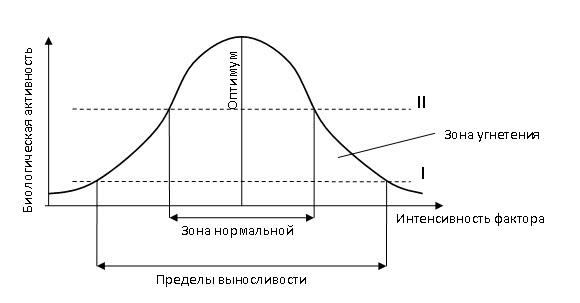
\includegraphics[width=\textwidth]{images/survive-diag.jpg}
    \caption{Диаграмма выживания}
\end{figure}

\textbf{Толерантность} -- это способность организма выдерживать отклонения экологических факторов от оптимальных.

По реакции на изменения абиотических факторов организмы делятся на:
\begin{itemize}
    \item \textbf{пойкилобионтов} (выносливых, толерантных). Эти организмы при отклонении значений фактора от точки оптимума сразу же изменяют интенсивность жизнедеятельности (пассивный тип приспособления). Если благоприятные условия возвратятся, то экологическая потенция восстановится.
    \item \textbf{гомойобионтов}, способных поддерживать гомеостаз -- постоянство своих свойств. В определенном диапазоне изменений фактора они включают механизмы защиты от неблагоприятных воздействий.
\end{itemize}

\textbf{Гомеостаз} -- способность биологических систем противостоять изменениям и сохранять относительное динамическое постоянство своей структуры и свойств.

По диапазону изменения факторов, в котором возможно существование организма, выделяют:
\begin{itemize}
    \item \textbf{стенобионтов} -- организмов, способных существовать лишь при относительно постоянных условиях окружающей среды (узкие пределы толерантности);
    \item \textbf{эврибионтов} -- организмов, способных существовать при значительных изменениях условий окружающей среды (широкие пределы толерантности).
\end{itemize}

\subsection{Совместное действие абиотических факторов}

В естественных условиях на живые организмы всегда действует не один, а сложный комплекс факторов. Для существования организма необходимо оптимальное сочетание факторов, но в природе не все они представлены оптимальными значениями. \textbf{Экологический оптимум} сочетания факторов отличается от оптимума какого-нибудь одного фактора.

\textbf{Закон минимума Либиха}. Для выживания организма (или экосистемы) наиболее значимым является тот экологический фактор, который наиболее удаляется (отклоняется) от своего оптимального значения.

\textbf{Закон толерантности Шелфорда} (является следствием закона Либиха). Существование экологического вида или целой экосистемы определяется лимитирующими факторами, находящимися не только в минимуме, но и в максимуме.

\textbf{Закон оптимума}. У любого фактора в экологии есть определенные границы, только в рамках которых данных фактор имеет положительное влияние на живой организм. За рамками этих границ -- влияние фактора становится отрицательным.

\textbf{Э. Рюбелем} был установлен \textbf{закон} (эффект) \textbf{компенсации} (взаимозаменяемости) факторов: отсутствие или недостаток некоторых экологических факторов может быть компенсировано другим близким (аналогичным) фактором. Например, недостаток света может быть компенсирован для растения обилием диоксида углерода, а при построении раковин моллюсками недостающий кальций может заменяться на стронций. Однако подобные возможности ограничены.

\textbf{В. Р. Вильямс} сформулировал \textbf{закон незаменимости фундаментальных факторов}: полное отсутствие в среде фундаментальных экологических факторов (света, воды, биогенов и т. д.) не может быть заменено другими факторами.

\textbf{Закон Митчерлиха-Бауле} (закон совокупного действия): в природе один экологический фактор может воздействовать на другой, поэтому успех вида в окружающей среде зависит от взаимодействия факторов. Повышенная температура способствует ускорению испарения влаги, животные труднее переносят высокие температуры при большой влажности. Совокупность факторов воздействуют сильнее всего на те фазы развития организмов, которые имеют наименьшую пластичность -- минимальную способность к приспособлению.

\subsection{Экологическая ниша}

Каждый вид адаптирован к строго определенной, специфичной для него совокупности условий существования -- экологической нише.

\textbf{Экологическая ниша} -- это совокупность всех требований организма к условиям среды обитания (составу и режимам экологических факторов) и места, где эти требования выполняются.

\textbf{Экологическая ниша} -- это совокупность всего множества биологических характеристик и физических параметров среды, определяющих условия существования того или иного вида, преобразования им энергии, обмен информации со средой и себе подобными.

\textbf{Местообитание} -- пространственно ограниченная совокупность условий среды (абиотической и биотической), обеспечивающая весь цикл развития и размножения особей (или группы особей) одного вида.

\textbf{Экологическая ниша} характеризует степень биологической специализации вида. Можно утверждать, что местообитание организма -- это его <<адрес>>, тогда как экологическая ниша -- его <<род занятий>>, или <<стиль жизни>>, или <<профессия>>.

\textbf{Принцип конкурентного взаимодействия Гаузе}: Два вида не занимают одну и ту же экологическую нишу. Пустующая экологическая ниша всегда и обязательно будет заполнена.

\textbf{Специализированные ниши}. Большинство видов растений и животных приспособлены к существованию в узком диапазоне климатических условий и иных характеристик окружающей среды, питаются ограниченным набором растений и животных. Такие виды имеют специализированную  нишу, определяющую их местообитание в природной среде. Так, гигантская панда на 99\% питается листьями и побегами бамбука.

\textbf{Общие ниши}. Для видов с общими нишами характерна хорошая приспосабливаемость к изменениями экологических факторов. Они могут успешно существовать в разнообразных местах, питаться различной пищей и выдерживают резкие колебания природных условий. Общие экологические ниши имеются у мух, тараканов, мышей, крыс, людей и т. д.

Для видов, имеющих общие экологические ниши, существует значительно меньшая угроза вымирания, чем для имеющих специализированные ниши.

\section{Популяционная экология (демэкология)}

\textbf{Популяция} -- это элементарная группировка организмов определенного вида, обладающая всеми необходимыми условиями для поддержания своей численности необозримо длительное время в постоянно изменяющихся условиях среды (С. С. Шварц, 1980).

С. С. Четвериковым (1903) сформулировано правило объединения в популяции: индивиды любого вида живого всегда представлены в в природной среде не изолированными отдельностями, а только их определенным образом организованными совокупностями.

Термин <<популяция>> в настоящее время используют в узком смысле слова, когда говорят о конкретной внутривидовой группировке, населяющей определенный биогеоценоз, и широком, общем смысле, для обозначения обособленной группы вида независимо от того, какую территорию она занимает и какую генетическую информацию несет.

Популяция является генетической единицей вида, изменения которой осуществляет эволюция вида. Как группа совместно обитающих особей одного вида, популяция выступает \textbf{первой надорганизменной биологической макросистемой}. У популяции приспособительные возможности значительно выше, чем у слагающих ее индивидов.

Пространство или ареал, занимаемое популяцией, может быть различным как для разных видов, так и в пределах одного вида. Величина ареала популяции определяется в значительной мере подвижностью особей или радиусом индивидуально активности. Если радиус индивидуальной активности невелик, величина популяционного ареала обычно также невелика.

Количество элементарных популяций, на которые распадается вид, зависит от разнородности условий среды обитания: чем они однообразнее, тем меньше элементарных популяций, и наоборот. Между элементарными популяциями всегда имеются некоторые отличия, появляющиеся в генетическом своеобразии, фенологических особенностях, интенсивности обмена, характере поведения.

Каждая элементарная популяция морфофизиологически и этологически (поведенчески) специфична, различия между ними определяются их генетическим своеобразием и средой обитания. Однако нередко смещение особей элементарных популяций, происходящие в природе, стирает границу между ними.

\textbf{Биологический полиморфизм} -- изменчивость, охватывающая в рамках популяции целые группы организмов, и сказывающаяся как на морфологии, так и на биологических свойствах.

\subsection{Характеристики популяции}

Статические или биологические свойства присущи как популяции, так и составляющим ее особям. Эти свойства характеризуют жизненный цикл  популяции. Популяция имеет определенную организацию и структуру, которую можно описать.

\noindent Выделяют следующие статические характеристики:
\begin{itemize}
    \item \textbf{Численность} --  число особей данного вида, полученное при пересчете тем или иным методом (тотальный учет, пробные площадки, метод мечения).
    \item \textbf{Биомасса} -- суммарный вес популяции, для животных это сумма веса всех организмов, для растений -- урожай на корню.
    \item \textbf{Плотность} -- численность или биомасса популяции, отнесенная к некоторой единице пространства. Обычно ее выражают числом особей или биомассой популяции на единицу площади или объема.
    \item \textbf{Плотность средняя} -- численность или биомасса, отнесенная ко всему пространству.
    \item \textbf{Плотность удельная} -- то же, но отнесенная к единице обитаемого фактически в данный момент пространства.
\end{itemize}

Размеры популяции уменьшаются в результате эмиграции и смертности. Таким образом,

Изменение численности популяции = (Рождаемость + Иммиграция) - (Смертность + Эмиграция).

\subsection{Возрастная структура}

Формирование возрастной структуры происходит в результате совместного действия процессов размножения и смертности.

В растущих популяциях рождаемость превышает смертность, численность увеличивается. В стабильной популяции рождаемость равна смертности, численность популяции почти не меняется, разновозрастные группы находятся примерно в одинаковом соотношении. Анализ возрастной структуры позволяет прогнозировать численность популяций на ряд ближайших поколений и лет, что применяется, к примеру, для оценки возможностей промысла рыбы, в охотничьем хозяйства, в некоторых зоологических исследованиях.

\subsection{Половой состав}

Первичное соотношение полов определяется генетическими механизмами -- равномерностью расхождения половых хромосом. Вторичное соотношение полов -- это соотношение полов на момент рождения (среди новорожденных). Третичное соотношение полов -- это соотношение полов среди взрослых животных.

\subsection{Пространственная структура}

Каждая популяция занимает пространство, обеспечивающее условия жизни для ограниченного числа особей. При изучении пространственной структуры различают случайное, равномерное и неравномерное (групповое) распределения особей на территории (в пространстве).

Равномерное распределение бывает там, где между особями очень сильна конкуренция или существует антагонизм (некоторые хищные рыбы). Наиболее часто наблюдается неравномерное (групповое) распределение -- образование различных скоплений. Случайное распределение в природе встречается редко, оно наблюдается в случаях, когда среда очень однородна и организмы не стремятся объединиться в группы.

В зависимости от характера использования пространства подвижных животных подразделяют на оседлых и кочевых.

\textbf{Оседлые} животные в течение всей или большей части жизни используют довольно ограниченный участок среды. Им присущи инстинкты привязанности к своему участку, регулярное возвращение к месту размножения после длительных и дальних миграций.

\textbf{Кочевые} животные совершают постоянные передвижения в пространстве, так как они зависят от запаса корма на данной территории. Кочевой образ жизни характерен преимущественно для стад и стай (кочующие группы многих рыб во время нагульных миграций, стада слонов, зебр, антилоп, северных оленей).

\subsection{Этологическая (поведенческая) структура}

Отражает разнообразные формы совместного существования особей в популяциях.

\textbf{Одиночный образ жизни} -- полностью одиночного существования организмов в природе нет, так как в этом случае было бы невозможно размножение.

\textbf{Семейный образ жизни} -- усиливаются связи между родителями и потомством, начинает заметно проявляться территориальное поведение животных. Путем различных сигналов, маркировки, угроз и тому подобного обеспечивается владение участком, достаточным для выкармливания потомства.

\textbf{Стая} -- временное объединение животных, проявляющих биологически полезную организованность действий (для защиты от врагов, добычи пищи, миграции и т. п.). Наиболее широко стайность распространена среди рыб и птиц, хотя встречается и у млекопитающих (собаки).

\textbf{Стадо} -- длительное или постоянное объединение животных, в котором осуществляется все основные функции жизни вида: добывания корма, защита от хищников, миграция, размножение, воспитание молодняка. Основу группового поведения в стадах составляют взаимоотношения доминирования (вожаки).

\textbf{Колония} -- групповое поселение оседлых животных на длительное время или период размножения. По сложности взаимоотношений между особями колонии очень разнообразны, наиболее сложные отношения складываются в поселениях для общественных насекомых (термитов, муравьев, пчел, ос и др.), возникающие на основе сильно разросшейся семьи. Члены колоний постоянно обмениваются информацией друг с другом.

\subsection{Динамические характеристики}

\textbf{Рождаемость и смертность}. Динамика численности и плотности популяций находятся в тесной зависимости от рождаемости и смертности.

\textbf{Рождаемость} -- это способность популяции к увеличению численности. Характеризует частоту появления новых особей в популяции. Различают рождаемость абсолютную и удельную. \textbf{Абсолютная} (общая) рождаемость -- число новых особей, появившихся за единицу времени. \textbf{Удельная} рождаемость выражается в числе особей на особь в единицу времени.

В популяции имеется тенденция к образованию теоретически максимально возможного количества новых особей. Оно достигается в идеальных условиях, когда отсутствуют лимитирующие экологические факторы и размножение ограничено лишь физиологическими особенностями вида. Обычно существует экологическая или реализуемая рождаемость, возникающая в обычных или специфических условиях среды. Средняя величина плодовитости выработана исторически как приспособление, которое обеспечивает пополнение убыли популяций. Численность и плотность популяции зависит и от ее смертности.

\textbf{Смертность популяции} -- это количество особей, погибших за определенный период. \textbf{Абсолютная} (общая) смертность -- это число особей, погибших в единицу времени. \textbf{Удельная смертность} -- это отношение абсолютной смертности к численности популяции. Абсолютная и удельная смертность характеризуют скорость убывания численности популяции вследствие гибели особей от хищников, болезней, старости и т. д.

Различают три типа смертности. Первый тип характеризуется одинаковой смертностью во всех возрастах. Данный тип смертности встречается редко и только у популяций, которые постоянно находятся в оптимальных условиях.

Второй тип характеризуется повышенной гибелью особей на ранних стадиях развития и свойственен большинству растений и животных.

Максимальная гибель животных происходит в личиночной фазе или в молодом возрасте, у многих растений -- в стадии произрастания семян и всходов. У насекомых до взрослых особей доживает 0.3 -- 0.5 \% отложенных яиц, у многих рыб 1 -- 2\% количества выметанной икры.

Третий тип отличается повышенной гибелью взрослых, в первую очередь, старых, особей. Отличается он у насекомых, личинки которых обитают в почве, воде, древесине, а также в других местах с благоприятными условиями.

\subsection{Рост популяции и кривые роста}

Если при незначительной эмиграции и иммиграции рождаемость превышает смертность, то популяция будет расти. Рост популяции является непрерывным процессом, если в ней существуют все возрастные группы.

При отсутствии каких-либо экологических ограничений рост происходит сначала медленно, а затем стремительно увеличивается по экспоненциальному закону. Такая модель основывается на допущении, что рост популяции не зависит от ее плотности. Считается, что почти любой вид при благоприятных условиях теоретически способен увеличить свою численность до заселения всей Земли. Первоначальный экспоненциальный рост в исходных благоприятных условиях со временем постепенно замедляется.

В природе рост популяции всегда ограничен рядом факторов: недостаток пищевых ресурсов, неблагоприятные погодные условия, хищничество, паразитизм, накопление токсичных продуктов метаболизма. Плотность популяции регулирует комплекс факторов, действующих на ее рост. С увеличением плотности скорость роста популяции постепенно снижается до нуля, и кривая выходит на некоторый стабильный уровень (плато).

\subsection{Колебания численности популяции}

Любые изменения популяции есть результат нарушения равновесия между ее биотическим потенциалом и сопротивлением окружающей среды. По достижении заключительной фазы роста размеры популяции продолжают колебаться от поколения к поколению вокруг некоторой более или менее постоянной величины. При этом численность одних видов изменяется нерегулярно с большой амплитудой колебаний (насекомые-вредители, сорняки), колебания численности других (например, мелких млекопитающих) имеют относительно постоянный период, а в популяциях третьих видов численность колеблется от года к году незначительно (долгоживущие крупные позвоночные и древесные растения).

\section{Экосистема}

\subsection{Основные понятия}

\textbf{Экологическая система} (экосистема) -- это совокупность живых организмов, взаимодействующих между собой и средой их обитания таким образом, что эта совокупность сохраняется неопределенно долгое время. Термин <<экосистема>> введен в 1935 г. английским экологом и геоботаником А. Тенсли.

\textbf{Биогеоценоз} (bios -- жизнь, гео -- Земля, ценоз -- сообщество) по В. Н. Сукачеву -- это совокупность природных элементов (атмосферы, горных пород, гидрологических условий, почвы, растительности, животных, микроорганизмов и др.) на определенном участке поверхности Земли. Контур биогеоценоза устанавливается по границе растительного сообщества (фитоценоза).

\textbf{Биоценоз} -- компонент биогеоценоза, включающий живые организмы (бактерии, растения, грибы, животные).

Термин <<экологическая система>> и <<биоценоз>> -- \textbf{не синонимы}.

\textbf{Экосистема} -- это любая совокупность организмов и среды их обитания, в том числе -- горшок с цветком, муравейник, болото, лес, пилотируемый космический корабль.

\textbf{Биогеоценозы} -- это только природные образования. Однако, биогеоценоз в полной мере может рассматриваться как экосистема.

Таким образом, понятие <<экосистема>> шире и полностью охватывает понятие <<биогеоценоз>> или <<биогеоценоз>> -- это частный случай <<экосистемы>>.

Экосистемный подход шире и учитывает общность организации всех природных систем независимо от местообитания.

Среди существующих на Земле экосистем выделяют:
\begin{itemize}
    \item микроэкосистемы (например, ствол гниющего дерева);
    \item мезоэкосистемы (например, лес, пруд и т. д.);
    \item макроэкосистемы (например, континент, океан и др.);
    \item глобальную (биосфера).
\end{itemize}

\subsection{Биомы}

Крупные наземные экосистемы называют \textbf{биомами}. Каждый биом включает в себя целый ряд меньших по размерам, связанных друг с другом экосистем.

Примеры природных экосистем и биомов по Одуму 1986 г. (наземные биомы):
\begin{itemize}
    \item вечнозеленый тропический дождевой лес;
    \item полувечнозеленый тропический лес с выраженными влажным и сухим сезоном;
    \item пустыня: травянистая и кустарниковая;
    \item чапараль -- районы с дождливой зимой и засушливым летом;
    \item тропические граследн и саванна;
    \item степь умеренной зоны;
    \item листопадный лес умеренной зоны;
    \item бореальные хвойные леса;
    \item тундра: арктическая и альпийская.
\end{itemize}
Типы пресноводных экосистем:
\begin{itemize}
    \item лентические (стоячие воды): озера, пруды и т. д.;
    \item лотические (текучие воды): реки, ручьи и т. д.;
    \item заболоченные угодья: болта, болотистые леса и т. д.
\end{itemize}
Типы морских экосистем:
\begin{itemize}
    \item открытый океан (пелагическая);
    \item воды континентального шельфа (прибрежные воды);
    \item районы апвеллинга (плодородные районы с продуктивным рыболовством);
    \item эстуарии (прибрежные бухты, проливы, устья рек, соленые марши).
\end{itemize}

Наземные биомы выделены по естественным или по исходным чертам растительности, а типы водных экосистем по геологическим и физическим особенностям.

Экосистемы не разбросаны в беспорядке, а сгруппированы в достаточно регулярных зонах как по горизонтали (по широте), так и по вертикале (по высоте). Впервые закономерность географической зональности на примере почв была сформулирована Докучаевым.

\textbf{Периодический закон географической зональности Григорьева-Будыко}: со сменой физико-географических поясов Земли аналогичные ландшафтные зоны и их некоторые общие свойства периодически повторяются, по этому принципу располагаются биомы. Повторение обусловлено одинаковым соотношением тепла и влаги наряду с различиями, обусловленными абсолютными значениями радиационного баланса. Величины индекса сухости меняются в разных зонах от 0 до 4-5.

\begin{figure}[H]
    \centering
    \includegraphics[width=0.9\textwidth]{images/bioms-law.png}
\end{figure}

\subsection{Экотон}

\textbf{Экотон} -- это зона напряжения, любая совокупность организмов и среды их обитания, где происходит и их взаимопроникновение. Экотон может иметь значительную линейную протяженность, но всегда бывает уже территории соседних сообществ. Примеры: переходная зона между лугом и агроценозом, эстуарий, лесостепь.

Правило экотона, или \textbf{краевого эффекта}: на стыках экосистем увеличивается число видов и особей в них, так как возрастает число экологических ниш из-за возникновения на стыках новых системных свойств.

\subsection{Автотрофы и гетеротрофы}

Живые организмы в экосистеме выполняют различные функции, которые зависят от типов питания. В ходе эволюции на Земле возникло два основных типа питания -- автотрофное и гетеротрофные.

\textbf{Продуценты} -- производители первичной продукции, синтезирующие органические вещества из неорганических соединений. Примеры: наземные зеленые растения, водоросли, фотосинтезирующие и хемосинтезирующие бактерии.

\textbf{Консументы} -- потребители органических веществ. Примеры: растительноядные (коза, гусеница), плотоядные (хищники), всеядные (человек).

\textbf{Редуценты} (деструкторы) -- восстановители. Трансформируют органические вещества отмерших организмов до простых неорганических соединений (углекислый газ, воду и др.), возвращая в почву или в водную среду биогенные элементы. В основном редуцентами являются бактерии и грибы.

\subsection{Экологические пирамиды}

\textbf{Экологические пирамиды} -- это графические модели, отражающие число особей (пирамида чисел), количество их биомассы (пирамида биомасс) или заключенной в них энергии (пирамида энергии) на каждом трофическом уровне и указывающие на понижение всех показателей с повышением трофического уровня.

Принцип построения экологических пирамид:
\begin{itemize}
    \item основание пирамиды образуют продуценты (растения);
    \item над ними располагаются консументы первого порядка (травоядные);
    \item следующий уровень представляют консументы второго порядка (хищники);
    \item и так далее до вершины пирамиды, которую занимают наиболее крупные хищники;
    \item высота пирамиды обычно соответствует длине пищевой цепи.
\end{itemize}

Пирамиды чисел отражают только плотность населения организмов на каждом трофическом уровне, но не скорость возобновления (оборота) организмов.

Правило экологической пирамиды биомасс отражает закономерность, согласно которой в любой экосистеме биомасса каждого следующего звена в 10 раз меньше предыдущего.

Если скорость размножения популяции жертвы высока, то даже при низкой биомассе такая популяция может быть достаточным источником пищи для хищников, имеющих более высокую биомассу, но низкую скорость размножения. По этой причине пирамиды численность \textbf{могут быть перевернутыми}, то есть плотность организмов в данной конкретный момент времени на низком трофическом уровне может быть ниже, чем плотность организмов на высоком уровне. Например, на одном дереве может жить и кормиться множество насекомых.

Перевернутая пирамида биомасс свойственна морским экосистемам, где первичные продуценты (водоросли планктона) очень быстро делятся (имеют большой репродуктивный потенциал и быструю смену поколений). В океане за год может смениться до 50 поколений фитопланктона. Потребители фитопланктона гораздо крупнее, но размножаются значительно медленнее. За то время, пока хищные рыбы (а тем более моржи и киты) накопят свою биомассу, сменится множество поколений организмов фитопланктона, суммарная биомасса которых намного больше.

Пирамидами биомасс не учитывается продолжительность существования поколений особей на разных трофических уровнях и скорость образования и выедания биомассы.

Универсальным способом выражения трофической структуры экосистем являются пирамиды скоростей образования живого вещества, то есть продуктивности. Их обычно называют пирамидами энергий, имея в виду энергетическое выражение продукции.

Пирамида энергии -- величина потока энергии, проходящего через различные трофические уровни. В отличие от пирамид чисел и биомасс, характеризующих статику экосистемы, пирамида энергии характеризует динамику прохождения массы пищи через пищевую цепь. На ее форму не влияют ни размеры особей, ни интенсивность их метаболизма. Кроме того, пирамида чисел преувеличивает роль мелких организмов, пирамида биомассы преувеличивает роль крупных. Поэтому пирамида энергии является наиболее универсальной характеристикой для сравнения потока энергии, проходящего через разные уровни, а также для сравнения одной экосистемы с другой.

Причины снижения количества энергии при переходе с одного трофического уровня на другой:
\begin{itemize}
    \item часть заключенной в пище энергии теряется в процессе биохимической трансформации пищи;
    \item часть энергии не усваивается и выводится из организма с экскрементами, а затем разлагается деструкторами;
    \item не все организмы данного трофического уровня будут съедены потенциальными хищниками и, следовательно, не вся энергия, запасенная в тканях, перейдет на следующий трофический уровень;
    \item часть энергии теряется в виде тепла в процессе дыхания;
    \item много энергии, полученной с пищей, тратится на работу, которую выполняет животное, перемещаясь, охотясь, строя гнездо или производя иные действия, в результате чего выделяется тепло.
\end{itemize}

\subsection{Первичная и вторичная продукция}

\textbf{Фотосинтез} -- это химическая реакция, которая протекает за счет солнечной энергии при участии хлорофилла (зеленые растения, бактерии -- пурпурные, зеленые, цианобактерии).
\[
    n\text{CO}_2 + n\text{H}_2\text{O} + \text{энергия} = \text{C}_n\text{H}_{2n}\text{O}_n + n\text{O}_2
\]

Глюкоза -- простейший продукт фотосинтеза:
\[
    6\text{CO}_2 + 6\text{H}_2\text{O} = \text{C}_6\text{H}_{12}\text{O}_6 + 6\text{O}_2.
\]

\textbf{Хемосинтез} -- процесс образования органических веществ из диоксида углерода за счет энергии, полученной при окислении неорганических соединений (аммиака, водорода, соединений серы, закисного железа и др.). Осуществляется некоторыми бактериями (железобактерии, серобактерии, нитрифицирующие бактерии, архен).

Согласно второму закону термодинамики (закон энтропии), процессы, связанные с превращением энергии, могут происходить самопроизвольно только при условии, что энергия переходит из концентрированной формы в рассеянную (деградирует). Для совершения жизненных процессов энергия солнечного излучения накапливается в экосистеме против термодинамического градиента.

Суть фотосинтеза -- увеличение свободной энергии в органическом веществе за счет преобразования энергии фотонов в энергию химических связей.

\textbf{Продуктивность экосистемы} -- это накопление экосистемой органического вещества в процессе ее жизнедеятельности. Продуктивность экосистемы измеряется количеством органического вещества, создаваемого за единицу времени на единицу площади. Различают разные уровни продуцирования, на которых создается первичная и вторичная продукция. Органическая масса, создаваемая продуцентами в единицу времени, называется \textbf{первичной продукцией}, а прирост за единицу времени массы консументов -- \textbf{вторичной продукцией}.

Первичная продукция подразделяется на два уровня: \textbf{валовую} и \textbf{чистую} продукцию.

\textbf{Валовая первичная продукция} -- это общая масса валового органического вещества, создаваемая в единицу времени при данной скорости фотосинтеза, включая траты и выдыхание.

Часть валовой продукции, которая не израсходована <<на дыхание>>, называется \textbf{чистой первичной продукцией}. Она представляет собой величину прироста растений и именно эта продукция потребляется консументами и редуцентами.

Вторичная продукция \textbf{не делится} на валовую и чистую, так как консументы и редуценты, то есть гетеротрофы, увеличивают свою массу за счет первичной продукции, то есть используют ранее созданную продукцию.

Р. Уиттекер (1980) делит по продуктивности все сообщества на четыре класса:
\begin{enumerate}
    \item \textbf{Сообщества высшей продуктивности}, 3000-2000 г/\(\text{м}^2\)/год. Сюда относятся тропические леса, посевы риса и сахарного тростника. Запас биомассы в этом классе продуктивности весьма различен и превышает 50 кг/\(\text{м}^2\) в лесных сообществах и равен продуктивности у однолетних сельскохозяйственных культур.
    \item \textbf{Сообщества высокой продуктивности}, 2000-1000 г/\(\text{м}^2\)/год. В этот класс включены листопадные леса умеренной полосы, луга при применении удобрений, посевы кукурузы. Максимальная биомасса приближается к биомассе первого класса. Минимальная биомасса соответственно равна чистой биологической продукции однолетних культур.
    \item \textbf{Сообщества умеренной продуктивности}, 1000-250 г/\(\text{м}^2\)/год. К этому классу относится основная масса возделываемых сельскохозяйственных культур, кустарники, степи. Биомасса степей меняется в пределах 0.2-5 кг/\(\text{м}^2\).
    \item \textbf{Сообщества низкой продуктивности}, ниже 250 г/\(\text{м}^2\)/год -- пустыни, полупустыни (в отечественной литературе их чаще называют опустыненными степями), тундры.
\end{enumerate}

Общая годовая продуктивность сухого органического вещества на Земле составляет 150-200 млрд т. Две трети его образуется на суше, третья часть -- в океане.

Вторичную продукцию рассчитывают отдельно для каждого трофического уровня, так как она формируется за счет энергии, поступающей с предыдущего уровня.

Все живые компоненты экосистемы -- продуценты, консументы и редуценты -- составляют общую биомассу сообщества в целом или его отдельных частей -- тех или иных групп организмов.

\end{document}
